\section{Cơ sở lý thuyết và công cụ}

\subsection{Cơ sở lý thuyết}

\subsubsection{Các bài toán NLP cơ bản}
\begin{itemize}
\item \textbf{Tách câu và mệnh đề (Clause Segmentation):}
Trong văn bản pháp lý, các điều khoản thường chứa câu phức với nhiều mệnh đề phụ hoặc danh sách liệt kê. Việc phân tách câu (segmentation) nhằm chia nhỏ văn bản thành các đơn vị ý nghĩa độc lập, tạo tiền đề cho các bước phân tích sau. Trong đồ án này, bài toán tách câu được mô hình hóa dưới dạng bài toán gán nhãn chuỗi (Sequence Labeling), xác định ranh giới mệnh đề kết hợp với xử lý luật (Rule-based) để tái tạo lại câu hoàn chỉnh.
\item \textbf{Phân cụm danh từ (Noun Phrase Chunking):}
Phân cụm danh từ là quá trình nhóm các từ liền kề nhau thành một cụm từ có chức năng như một danh từ trong câu. Quá trình này thường sử dụng lược đồ gán nhãn BIO (Begin - Inside - Outside) hoặc IOB2. Cụ thể, 'B-NP' đánh dấu từ bắt đầu cụm, 'I-NP' đánh dấu các từ bên trong cụm, và 'O' đánh dấu các từ nằm ngoài cụm.
\item \textbf{Phân tích cú pháp phụ thuộc (Dependency Parsing):}
Phân tích phụ thuộc là việc xác định các mối quan hệ ngữ pháp giữa các từ trong một câu. Cấu trúc này được biểu diễn dưới dạng một cây có hướng, trong đó một từ đóng vai trò là từ trung tâm (head) và các từ khác là phụ thuộc (dependent) với một nhãn quan hệ cụ thể (ví dụ: \textit{nsubj} - chủ ngữ, \textit{obj} - tân ngữ, \textit{root} - động từ chính).
\end{itemize}

\subsubsection{Trích xuất Thông tin và Ngữ nghĩa}
\begin{itemize}
\item \textbf{Nhận dạng thực thể có tên (Named Entity Recognition - NER):}
NER là tác vụ trích xuất và phân loại các cụm từ quan trọng trong văn bản vào các danh mục định trước. Đối với miền pháp lý, lược đồ thực thể tùy chỉnh thường phức tạp hơn, bao gồm: \textit{PARTY} (Chủ thể), \textit{MONEY} (Số tiền), \textit{DATE} (Thời gian), \textit{PENALTY} (Điều khoản phạt), \textit{LAW} (Luật áp dụng)... Mô hình NER thường được giải quyết bằng các kiến trúc học sâu như BiLSTM-CRF hoặc các mô hình ngôn ngữ lớn dựa trên Transformer.

\item \textbf{Gán nhãn vai trò ngữ nghĩa (Semantic Role Labeling - SRL):}
SRL nhằm mục đích trả lời câu hỏi "Ai làm gì cho ai, ở đâu, khi nào, và như thế nào?" đối với mỗi vị ngữ (predicate) trong câu. Các vai trò ngữ nghĩa (Arguments) thường bao gồm: \textit{Agent} (tác nhân gây ra hành động), \textit{Theme} (đối tượng chịu tác động), \textit{Recipient} (người nhận), và \textit{Time/Location} (thời gian/địa điểm). Trong bài tập lớn này, SRL kết hợp đặc trưng từ NER và Dependency Parsing để tăng cường độ chính xác.

\item \textbf{Phân loại ý định (Intent Classification):}
Đây là bài toán phân loại câu (Text Classification) nhằm gán nhãn chức năng pháp lý cho một điều khoản. Các nhãn thường bao gồm: \textit{Obligation} (Nghĩa vụ), \textit{Prohibition} (Điều cấm), \textit{Right} (Quyền lợi) và \textit{Termination Condition} (Điều kiện chấm dứt). Bài toán có thể giải quyết bằng các phương pháp Machine Learning truyền thống (TF-IDF kết hợp Logistic Regression) hoặc tinh chỉnh (fine-tune) các mô hình Transformer.
\end{itemize}


\subsubsection{Mô hình ngôn ngữ Transformer và PhoBERT}
\begin{itemize}
\item \textbf{Kiến trúc Transformer:}
Khác với RNN/LSTM truyền thống xử lý dữ liệu tuần tự, Transformer sử dụng cơ chế tự chú ý (Self-Attention) cho phép mô hình nhìn vào toàn bộ ngữ cảnh của câu cùng một lúc, giải quyết triệt để vấn đề phụ thuộc xa (long-term dependency) và cho phép huấn luyện song song \autocite{vaswani}.

\item \textbf{PhoBERT:}
PhoBERT \autocite{phobert} là mô hình ngôn ngữ tiền huấn luyện (Pre-trained Language Model) dựa trên kiến trúc RoBERTa, được huấn luyện đặc biệt cho tiếng Việt với kho dữ liệu khổng lồ (20GB văn bản thô). Việc fine-tune PhoBERT mang lại hiệu quả vượt trội cho các tác vụ hiểu ngôn ngữ tự nhiên tiếng Việt như NER, SRL và Text Classification. Trong dự án, để chống lại nhiễu dữ liệu và giảm overfitting, kỹ thuật \textit{Multi-Sample Dropout} \autocite{multidrop} được tích hợp vào kiến trúc phân loại của PhoBERT.
\end{itemize}


\subsubsection{Hệ thống Hỏi đáp kết hợp Truy xuất (Retrieval-Augmented Generation - RAG)}

RAG là một kiến trúc kết hợp giữa khả năng truy xuất thông tin truyền thống (Information Retrieval) và khả năng sinh văn bản của Mô hình Ngôn ngữ Lớn (LLM). Thay vì dựa hoàn toàn vào tham số nội tại, RAG truy xuất các tài liệu/mệnh đề có liên quan nhất từ một Cơ sở dữ liệu Vector (Vector Database) dựa trên câu hỏi của người dùng. Các tài liệu này sau đó được ghép vào ngữ cảnh (context prompt) để LLM sinh ra câu trả lời chính xác, có cơ sở và giảm thiểu tối đa hiện tượng "ảo giác" (hallucination) \autocite{retrieval}.

% [Placeholder: Hình minh họa kiến trúc RAG]
\begin{figure}[H]
    \centering
    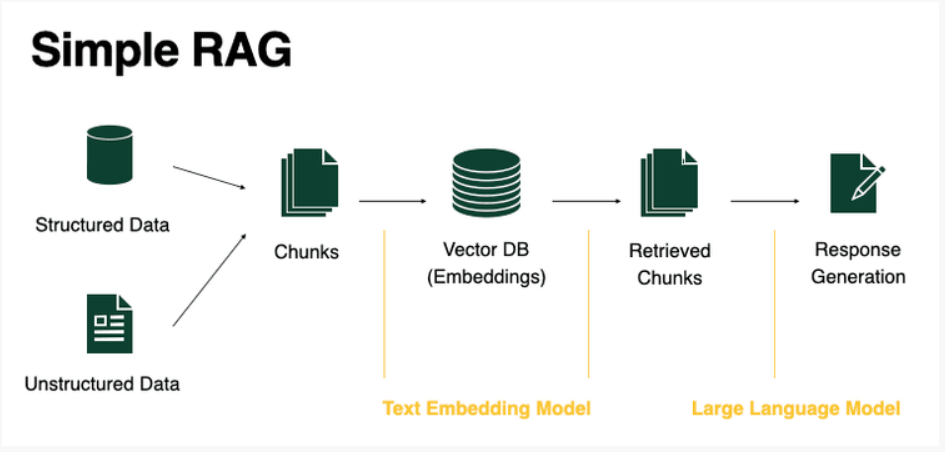
\includegraphics[width=1.0\textwidth]{Image/simple_rag.png}
    \caption{Kiến trúc tổng quan của hệ thống RAG. Nguồn: \href{https://www.bentoml.com/blog/building-rag-with-open-source-and-custom-ai-models}{Simple RAG}.}
    \label{fig:rag_arch}
\end{figure}

\subsection{Công cụ và thư viện}
Để triển khai hệ thống, đồ án sử dụng các công cụ và thư viện mã nguồn mở sau:
\begin{itemize}
    \item \textbf{Stanza \& Underthesea:} Các bộ công cụ NLP chuyên dụng. Underthesea được sử dụng để tách từ tiếng Việt (Word Segmentation), trong khi Stanza (phát triển bởi Stanford NLP) được cấu hình offline để phân tích cú pháp phụ thuộc (Dependency Parsing) và gán nhãn từ loại với độ chính xác cao.
    \item \textbf{HuggingFace Transformers \& PyTorch:} Nền tảng cốt lõi để tải, tinh chỉnh (fine-tune) và thực hiện suy diễn (inference) mô hình PhoBERT. Khung PyTorch cho phép tùy biến sâu các hàm mất mát (như \textit{Focal Loss}) và kiến trúc mạng học sâu bổ sung (như \textit{BiLSTM} cho tác vụ SRL).
    \item \textbf{ChromaDB:} Cơ sở dữ liệu Vector mã nguồn mở, được tích hợp qua LangChain, giúp lưu trữ embedding của các mệnh đề hợp đồng và siêu dữ liệu (metadata) hỗ trợ truy vấn lọc ngữ nghĩa tốc độ cao.
    \item \textbf{Google GenAI (Gemini 3.1 Flash):} API mô hình ngôn ngữ lớn đóng vai trò là khối sinh (Generator) trong pipeline RAG, cũng như góp phần hỗ trợ làm sạch/chuyển đổi văn bản hợp đồng thô ở khâu tiền xử lý một cách tự động.
    \item \textbf{FastAPI \& Streamlit:} FastAPI được dùng để xây dựng các API xử lý ngôn ngữ chịu tải cao, cung cấp backend kết nối với mô hình AI. Streamlit được dùng để xây dựng giao diện người dùng (UI) tương tác trực quan cho phép người dùng hỏi đáp và xem trực quan hóa kết quả phân tích NLP.
\end{itemize}